\indent 

Monte Carlo Method was invented by a Polish mathematician called Stanislaw Ulam in the late 1940s. Inspiration during recovery from illness with a thought experiment. Monte Carlo was the code name given for the project (Inspired by the Monte Carlo casino in Monaco where Ulam’s uncle would borrow family money to gamble).

Monte Carlo are a class of computational methods that can be applied to a wide range of problems. Key aspect of Monte Carlo methods are that they rely on \textbf{random sampling}. Generally provide approximate solutions, not exact solutions.

Used in cases where analytic solutions don’t exist or are too difficult to implement. Monte Carlo methods are sometimes referred to as stochastic simulation.

\begin{figure}[h!]
    \centering
    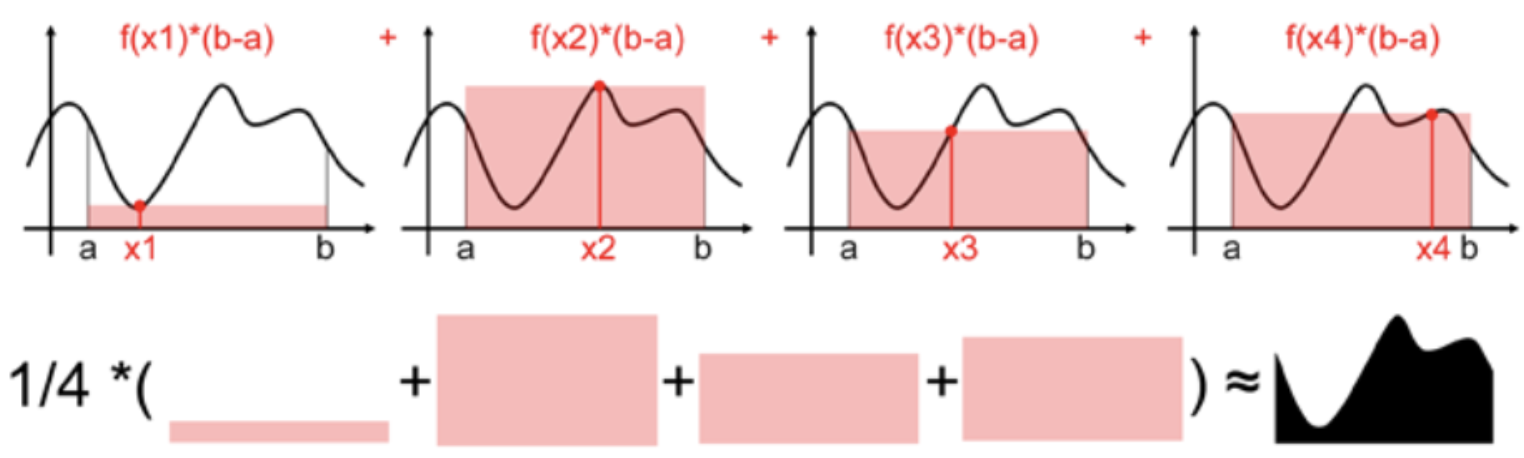
\includegraphics[width=0.9\linewidth]{Figure/Week 10/Monte Carlo visually.png}
    \caption{Monte Carlo visually}
\end{figure}

\subsection{Monte Carlo Methods}

\indent

\subsubsection{Monte Carlo estimation of $\pi$}

\indent 

Randomly draw $N$ points within unit square at random. Count the $R$ points which are inside the unit circle. Compute the ratio $R/N$ and estimate $\pi$ as $4R/N$.

In this example, the mathematical statistics of the procedure is:

Write the parameter we want to estimate, i.e., $pr$, as an expectation. Represent the parameter as a sample approximation. Let $f(\cdot)$ be the probability density function (pdf) of $X$ and $A$ be the support of $X$.

\begin{align*}
    \mathbb{E}[X] = \int _A tf(t)dt\approx \frac{1}{N}\sum_{i=1}^N X_i
\end{align*}

The law of large numbers guarantees that as the number of samples we draw increase, the estimator converges to the true parameter value almost surely.

We can replace $X$ with a function $g(X)$. Then the previous equation becomes:

\begin{align*}
    \mathbb{E}[g(X)] = \int_A g(t)\cdot f(t)dt\approx \frac{1}{N}\sum_{i=1}^N g(X_i)
\end{align*}

Here, we assume to draw $X_i \sim f$.

\subsubsection{Monte Carlo Integration example}

\indent 

One example is: $g(x) = e^{-x^2/2}$. $X_i$ is a uniform random variable on $(0,1)$. Then:

\begin{align*}
    \mathbb{E}[g(X)] = \int_0^1 e^{-x^2/2}dx\approx \frac{1}{N}\sum_{i=1}^N g(X_i)
\end{align*}

Goal is to evaluate the following definite integral: $\int_0^1 e^{-x^2/2}dx\approx \frac{1}{N}\sum_{i=1}^N g(X_i)$. Find a random variable such that the above holds. Need to be careful such that: Domain of the random variable and $g$ agree with the above definition.

\subsubsection{Simulating random variable}

\indent 

Let’s say we know how to simulate random variables that has a uniform distribution on the interval $[0,1]$. Call this uniformly distributed random variable $U$. Can do that in \texttt{R} with \texttt{runif}.

In \texttt{R}, we can draw random Gaussian variables using the function \texttt{rnorm}, but how do these functions really work? Two methods (others exist):

\begin{itemize}
    \item Inverse-transform method
    \item Acceptance-rejection method
\end{itemize}

Disadvantages of Simulating:

\begin{itemize}
    \item Inefficient when targeting rare events or small regions of the space.
    \item Scales poorly with dimensionality (curse of dimensionality)
    \item No adaptive as each sample is independent–no feedback or learning from previous samples.
\end{itemize}

\bigskip

\noindent \textbf{Inverse-transform method}:

Let’s say $X$ is a random variable that has a cumulative distribution function (cdf) $F$. Remember that cdf is the integral of the pdf:

\begin{align*}
    F(x) = \int_{-\infty}^x f(t)dt
\end{align*}

Recall $U$ is a uniformly distributed random variable over $[0,1]$. If the inverse of $F(x)$ exists, then we can generate $X$ as: $X=F^{-1}(U)$.

The exponential distribution has a pdf of the form:

\begin{align*}
f(x) = 
    \begin{cases}
        \lambda e^{-\lambda x} & \text{if } x>0\\
        0 & \text{if }x\leq 0
    \end{cases}
\end{align*}
    
and a cdf of the form:

\begin{align*}
F(x) = 
    \begin{cases}
        1- e^{-\lambda x} & \text{if } x>0\\
        0 & \text{if }x\leq 0
    \end{cases}
\end{align*}

The inverse cdf is:

\begin{align*}
    F^{-1}(p) = -\frac{\log(1-p)}{\lambda}, 0<p<1
\end{align*}

To sample from the exponential distribution, we can do the following:

\begin{itemize}
    \item Sample $U\sim \text{Uniform}(0,1)$
    \item Set $X = -\frac{\log(1-U)}{\lambda}$
\end{itemize}

\bigskip

\noindent \textbf{Acceptance-Rejection method}:

The problem with the inverse transform method is that you need to know the functional from of the inverse of the cdf. Acceptance-rejection method is a more general method can simulate “difficult” distributions.

Given two probability densities $f(x)$ and $g(x)$, with $f(x)<Mg(x)$ for all $x$. If $g(x)$ is a distribution that can be easily sampled, then we can sample $f(x)$ using the following procedure:

\step Draw a random variable $X\sim g(x)$.

\step Accept $X$ with probability $\frac{f(x)}{Mg(x)}$

\step Repeat steps 1 and 2 until you have the desired number of random samples

Problems with the Acceptance-rejection method: The envelop distribution $g(x)$ needs to closely resemble $f(x)$ for this method to work well.

If $g(x)$ does not match $f(x)$ well: The method will draw a lot of unwanted samples hence is not very efficient. Become very problematic when the data are high-dimensional. Even at dimensions of $\sim 10$, this method becomes very inefficient, i.e., you need to draw lots of samples before one sample is accepted.

\subsection{Monte Carlo simulation examples}

\subsubsection{Pop Mart Blind Box}

\indent 

Each Pop Mart Monster blind box costs \$22. There are 10 unique figures in the full set. Each box contains one random figure. How many boxes would you need to purchase — and how much money would you expect to spend — to collect all 10 figures?

\bigskip

\noindent\textbf{Analytical Solution (before we see the Monte Carlo)}:

Expected number of shops you need to do:

\begin{align*}
    \mathbb{E}[T] = n(\frac{1}{1}+\frac{1}{2}+\ldots + \frac{1}{n}) \approx n\log n+0.5772n+0.5
\end{align*}

where $T$ is the number of shops you need to do, and $n$ is the number of items to collect.

For the example, we have $n=10$ (the number of unique figures) so $E[T]≈30$. On average, you need to buy about 30 boxes.

\bigskip

\noindent\textbf{Monte Carlo Simulation}:

Using in \texttt{R}, the results is 29.733.

\subsubsection{Polya urn problem}

\indent

Let an urn start with 1 black ball and 1 white ball. Repeatedly draw a single ball from the urn. Each time a ball is drawn: You put back that ball plus one extra ball of the same colour back into the urn.

After 1000 draws, how many black balls do you expect to be in the urn? This is an example of using Monte Carlo to simulate a process.

\subsubsection{Call Option Pricing}

\indent

An European call option gives you the right to buy a stock at a particular price at expiry. 

Example: 90 day call option of a stock with \$105 strike. Let’s say a stock is currently priced at \$100. If it hits \$108 at day 90, then you can exercise the option and make a \$3 profit from this stock. If its price is below \$105 at day 90, then you make nothing.

Question: How much should you pay for this option today? Think of this as the insurance premium you’d pay to guarantee the right to buy later at a known price. A put option gives you the right to sell a stock at a particular price at expiry.

At expiration, the payoff of the call option is: $\text{Payoff} = \max (S_T - K,0)$, where $S_T$ is the stock price at expiry and $K$ is the strike price.

\noindent\textbf{Simulate stock price as a random (stochastic) model}:

Equation for the future price $S$ of a stock: $dS = S(\mu dT+\sigma\sqrt{dT}\mathcal{N})$, where $\mu$ is the growth rate of the stock price, $\sigma$ is known as the volatility (Think of this as the variance of the stock price), $\mathcal{N}$ is a standard normal random variable, $dT$ is one unit of time.

\noindent\textbf{Monte Carlo Simulation}:

\step Simulate many possible future stock prices $S_T$  based on the above equation.

\step For each simulation, calculate payoff.

\step The price you are willing to pay is the expected value of the payoff $E(\text{Payoff})$.

